\documentclass{standalone}
\usepackage[utf8]{inputenc}
\usepackage[T1]{fontenc}

\usepackage[margin=1in]{geometry}
\usepackage{tikz-qtree}
\usetikzlibrary{shadows,trees}
\begin{document}
\tikzset{font=\small,
level distance=.8cm,
every node/.style=
    {color=white,
    rectangle,rounded corners,
    align=center,
    text = black
    },
edge from parent/.style=
    {draw=blue,
    thick
    }}

\centering
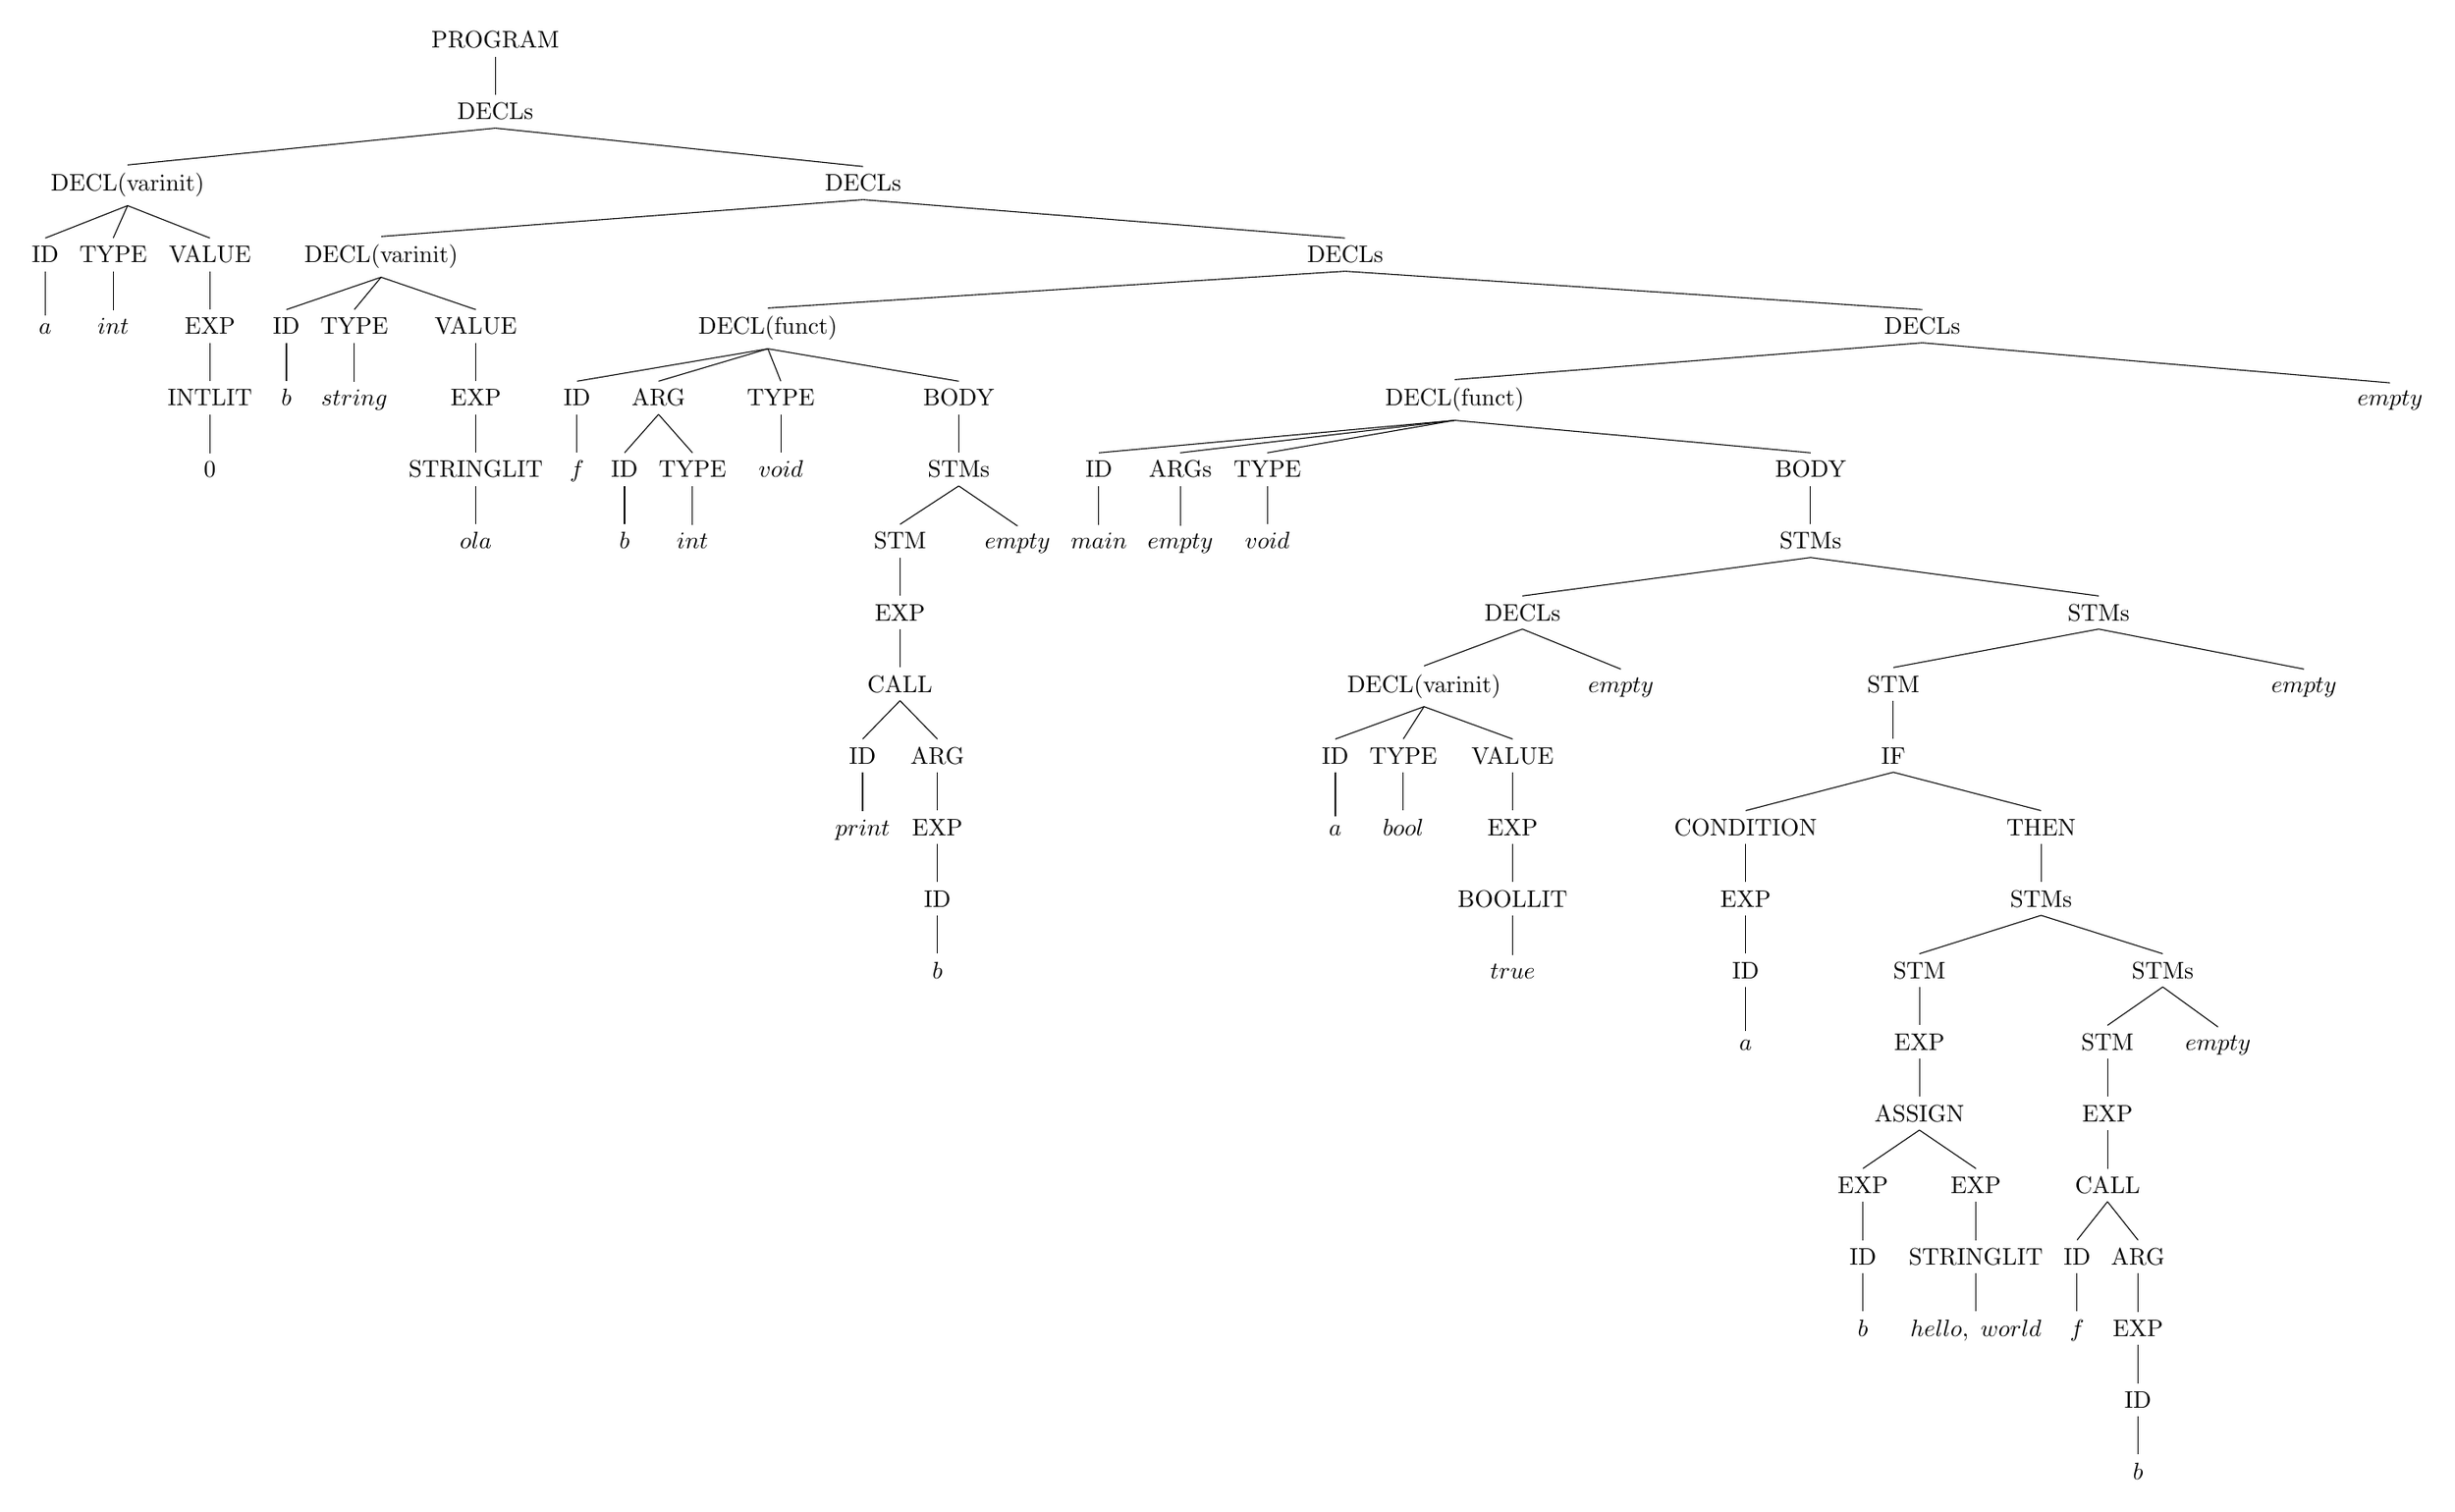
\begin{tikzpicture}
\Tree [.PROGRAM
[.DECLs [.DECL(varinit) [.ID $a$ ][.TYPE $int$ ]
[.VALUE [.EXP [.INTLIT $0$ ] ]
] ]
[.DECLs [.DECL(varinit) [.ID $b$ ][.TYPE $string$ ]
[.VALUE [.EXP [.STRINGLIT $ola$ ] ]
] ]
[.DECLs [.DECL(funct) [.ID $f$ ] [.ARG [.ID $b$ ] [.TYPE $int$ ]
]
[.TYPE $void$ ]
[.BODY [.STMs [.STM [.EXP [.CALL [.ID $print$ ] [.ARG [.EXP [.ID $b$ ] ]
]
] ]
]
$empty$ ]
] ]
[.DECLs [.DECL(funct) [.ID $main$ ] [.ARGs $empty$ ] [.TYPE $void$ ]
[.BODY [.STMs [.DECLs [.DECL(varinit) [.ID $a$ ][.TYPE $bool$ ]
[.VALUE [.EXP [.BOOLLIT $true$ ] ]
] ]
$empty$ ]
[.STMs [.STM [.IF [.CONDITION [.EXP [.ID $a$ ] ]
] [.THEN [.STMs [.STM [.EXP [.ASSIGN [.EXP [.ID $b$ ] ]
[.EXP [.STRINGLIT $hello,\ world$ ] ]
] ]
]
[.STMs [.STM [.EXP [.CALL [.ID $f$ ] [.ARG [.EXP [.ID $b$ ] ]
]
] ]
]
$empty$ ]
]
] ] ]
$empty$ ]
]
] ]
$empty$ ]
]
]
]
]
\end{tikzpicture}
\end{document}
